\documentclass[dvisvgm]{standalone}

\usepackage{tikz}
\usetikzlibrary {arrows.meta, positioning, automata}

\begin{document}

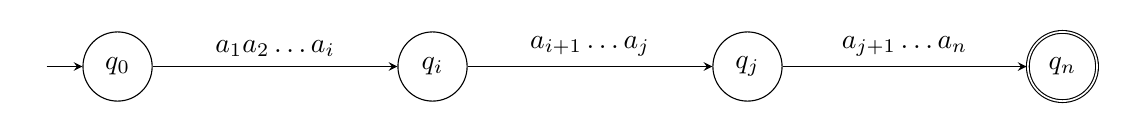
\begin{tikzpicture}[
    ->,
    >=stealth,
    node distance=4cm,
    initial text=$ $,
    on grid,
]

    \node[initial,   state]                    (A) {$q_0$};
    \node[           state, right =of A] (B) {$q_i$};
    \node[           state, right =of B] (C) {$q_j$};
    \node[accepting, state, right =of C] (D) {$q_n$};

    \path
        (A) edge [above]       node {$a_1a_2\dots a_i$}  (B)
        (B) edge [above]       node {$a_{i + 1}\dots a_j$}  (C)
        (C) edge [above]       node {$a_{j + 1}\dots a_n$}  (D)
    ;
\end{tikzpicture}

\end{document}